\chapter[\color{oxfordblue} Combined \boldvhbc\ Analysis]{\color{oxfordblue} Combined \vhbc\ Analysis}\label{chap-VH}
\ChapFrame

\textit{Perhaps the most important \textit{raison d'être} of the \textit{Large Hadron Collider} was to discover the Brout-Englert-Higgs boson (Higgs - $H$), a feat achieved by the ATLAS and CMS Experiments in July 2012 \cite{ATLAS:2012yve, CMS:2012qbp}. Theorised in 1964 by two independent papers introducing the mechanism of spontaneous symmetry breaking to give mass to the gauge bosons \cite{Englert:1964et,  PhysRevLett.13.508}, its discovery almost fifty years later marked one of the greatest achievements of the particle physics community. The Higgs boson is an essential part of the Standard Model. It is tied to the mechanism through which particles acquire mass without breaking the electroweak gauge invariance, as described in Chapter~\ref{chap-theory}. While the gauge bosons $W$ and $Z$ gain mass through symmetry breaking, in the \gls{sm} the fermions acquire theirs through Yukawa interactions with the Higgs fields \cite{10.1143/PTPS.1.1}. The scale of the interaction for each fermion $f$ is set by an associated Yukawa coupling $y_f$. These couplings are fundamental parameters of the \gls{sm} depending on the quark masses and the Higgs field vacuum expectation. This chapter is dedicated to an ATLAS measurement of the $y_b$ and a search of the $H \rightarrow c\bar{c}$ decay mode.}

\section{Introduction}
The Higgs boson $H$ \cite{Englert:1964et, PhysRevLett.13.508, Higgs:1964ia, PhysRevLett.13.585} was discovered in 2012 by the ATlAS and CMS Collaborations using the data of the \gls{lhc} Run 1 \cite{ATLAS:2012yve, CMS:2012qbp}. This triggered a race by both experiments to study the specific properties of the discovered particle, and in particular to observe the different production and decay modes presented in Chapter~\ref{th-sec-higphe}. The initial decay channels studied for the discovery were the bosonic decays of the Higgs to final states of photons and leptons: $H \rightarrow \gamma\gamma$, $H \rightarrow ZZ$, and $H \rightarrow WW$. These channels benefit from clean experimental conditions, reliable measurements, and limited backgrounds. The new particle is now being studied in ever finer detail, confirming its coupling to many massive particles of the \gls{sm} and showing remarkable agreement with the properties dictated by the theory. During the \gls{lhc} Run 2, corresponding to data taken from 2015 to 2018, the $t\bar{t}H$ production mechanism was observed for the first time, providing the first direct measurement of the top Yukawa coupling \cite{ATLAS:2018mme, CMS:2018uxb}. Additionally, the decay of Higgs bosons to a pair of $\tau$-lepton is now well established and different cross section measurements have been performed \cite{atlasTauMeasu, CMS:2021gxc}. Importantly, the decay channel of the Higgs boson to a $b\bar{b}$ pair was observed by both ATLAS and CMS \cite{ATLAS:2018kot, CMS:2018nsn}. This last decay channel is of particular significance since it has the largest predicted branching ratio of 58\% for an \gls{sm} Higgs with a mass of 125 GeV. \\ 

Concerning the second generation of fermions, there is 3 $\sigma$ evidence of the decay to a $\mu^-\mu^+$ pair by CMS \cite{CMS:2020xwi} and a 2 $\sigma$ excess over the background-only hypothesis by ATLAS \cite{ATLAS:2020fzp}. Additionally, constraints on the branching ratio of the $H$ to another second generation fermion, the $c$-quark, have been set by both Collaborations studying the $H \rightarrow c\bar{c}$ decay mode \cite{Aaboud:2018fhh}. This decay mode is the most common Higgs decay mode that has yet to be observed. It is particularly challenging due to the combination of a small predicted 2.9\% branching ratio \cite{DJOUADI199856}, large background rates, and the experimental difficulties in identifying $c$-jets. It is a fertile ground for new physics beyond the \gls{sm} due to the smallness of the predicted $c$-quark Yukawa coupling $y_c \approx 3.99 \times 10^{-3} $ \cite{yukawac} as well as an important test of the validity of the model \cite{PhysRevD.89.033014,PhysRevD.92.033016,Botella:2016krk,PhysRevD.98.055001,GHOSH2016504,PhysRevLett.123.031802,PhysRevD.100.115041}. The Yukawa couplings in the \gls{sm} are largely added ad-hoc and do not explain the distinct mass hierarchy between the three generations of fermions. This open problem is probed by studying the coupling strengths of the quarks to the Higgs boson. The $VH (H \rightarrow b\bar{b}/c\bar{c})$ analysis to which this chapter is dedicated scrutinises the hierarchy of mass between the $b$- and $c$-quark.

\section[The \vhb\ and \vhc\ ATLAS Analyses]{The \boldvhb\ and \boldvhc\ ATLAS Analyses}
While $H \rightarrow b\bar{b}$ enjoys the largest decay branching ratio at the observed Higgs mass, the large multi-jet background in a hadron collider makes this decay mode very challenging. The measurements for both the $b\bar{b}$ and $c\bar{c}$ decay modes are therefore performed in the \textit{associated production mode}, where the $H$ is produced in addition to an extra vector boson $V$ ($W$ or $Z$) decaying leptonically, to electrons ($e$), muons ($\mu$), neutrinos ($\nu$), or a combination $e\nu$ or $\mu\nu$. Despite the relatively small cross section of the $VH$ production mode ($\sigma_{VH}$ = 2.25 pb compared to the total $H$ production $\sigma_H \approx$ 51 pb), the process benefits from experimentally favourable conditions thanks to the presence of leptons in the event signature, allowing for efficient triggering and greatly reducing the contribution of the multi-jet background. Other analyses relying on full-hadronic final states in the associated or other production modes are also performed by the ATLAS Collaboration, but are less sensitive to the Higgs coupling to heavy-flavour quarks. The \vhb\ and \vhc\ ATLAS analyses adopt very similar strategies. The main ingredient is to reliably tag the flavour of jets produced in an event to reconstruct the heavy-quark pair produced in the $H$ decay, with the taggers described in Chapter \ref{chap-ftag}. \\ 

Using the Run 2 dataset with an integrated luminosity of 139 fb$^{-1}$, the published \vhc\ ATLAS analysis obtained an observed (expected) upper limits on the \vhc\ signal strength of 26 $\times$ \gls{sm} (31 $\times$ \gls{sm}) \cite{Collaboration:2721696}. The measurement also provided the first constraint on the Higgs-charm coupling modifier $|\kappa_c| < 8.5$. For comparison, CMS reported an observed (expected) upper limit of 14.4 $\times$ \gls{sm} (7.6 $\times$ \gls{sm}) and a constraint of $|\kappa_c| < 3.4 $ on the coupling modifier \cite{arXiv:2205.05550}. \\ 

For the $VH (H\rightarrow b\bar{b})$, thanks to a larger expected signal, the ATLAS analysis reaches a sensitivity of 6.7 standard deviations \cite{ATLAS:2020fcp}. Having reached the observation level, the focus for this channel is now to perform precision differential measurements of the fiducial cross sections as a function of momentum in the reduced \glsreset{stxs}\gls{stxs} scheme. To probe larger $p_T$ ranges, the analysis is now split into the \textit{resolved} \cite{ATLAS:2020fcp} and the \textit{boosted} \cite{ATLAS:2020jwz} analyses, with the latter restricting to values of the transverse momentum of the associated vector boson \ptv\ above 250 GeV - a property highly correlated to the \pt\ of the Higgs $p_T^H$. The name of these analyses comes from the strategy to reconstruct the Higgs boson candidate. At low \ptv, the two $b$-jets from the $H$ boson decay can be independently resolved into two distinct small cone radius (small-$R$) jets. At high \ptv, the $H$ boson is highly Lorentz-boosted and the candidate $H$ boson is efficiently reconstructed as a single large-radius ($R = 1$) jet merging the two $b$-jets. The measured signal strengths, defined as the ratio of the measured yield to the \gls{sm} predictions, are: 
\begin{itemize}
\item For the resolved analysis in Run 2: a signal strength of $1.02_{-0.17}^{+0.18}$ corresponding to an observed (expected) significance of 6.7 (6.7) standard deviations \cite{ATLAS:2020fcp}. Due to the good sensitivity of the analysis, the result is further detailed into the $WH$ and $ZH$ production processes with observed (expected) significances of, respectively, 4.0 (4.1) and 5.3 (5.1) standard deviations. Furthermore, the $VH$ cross section times the $H \rightarrow b\bar{b}$ and $V\rightarrow$ leptons branchings fractions ($\sigma \times BR$) are reported in the reduced \gls{stxs} scheme. Finally, limits are set on the coefficients of effective Lagrangian operators which can affect the $VH$ production and the $H \rightarrow b\bar{b}$ decay.
\item For the boosted analysis: a signal strength of  $0.72_{-0.36}^{+0.39}$ corresponding to an observed (expected) significance of 2.1 (2.7) standard deviations \cite{ATLAS:2020jwz}.
\end{itemize}

Some preliminary studies aiming at combining the different analyses have already been performed, with the resolved \vhb\ and \vhc\ analyses combined in Ref. \cite{Collaboration:2721696} and the resolved and boosted $VH (H \rightarrow b\bar{b})$ combined\footnote{CMS published an analogous combination in Ref. \cite{CMS-PAS-HIG-20-001}.} in Ref. \cite{ATLAS:2021wqh}. These combinations require careful studies to remove the overlap between the analyses. In this analysis, it was done by introducing a switch in \ptv\ at 400 GeV between the resolved and boosted strategies as adopted in the respective analyses. The objective of the combined analysis presented here is to define a common analysis strategy, correlating as much as possible the experimental and modelling uncertainties for both Higgs decay modes and \ptv\ regimes, thereby improving the measurements of $VH (H \rightarrow b\bar{b})$ and $VH (H \rightarrow c\bar{c})$ simultaneously. This new combined measurement strategy brings two main benefits: 
\begin{itemize}
\item The Higgs-charm and -beauty coupling modifiers, $\kappa_c$ and $\kappa_b$, can be measured directly, as well as their ratio $\kappa_c/\kappa_b$. 
\item The auxiliary measurements of background processes are shared, leading to a better constraining of important backgrounds such as the $V$+jets and top-quark processes.
\end{itemize}
The combined analysis also benefits from improved signal selections thanks to upgraded physics objects and event reconstruction techniques. In particular, new machine learning-based techniques are integrated for both the event selection, the discriminant, and flavour tagging.

This chapter details the current state of the $VH (H\rightarrow b\bar{b}/c\bar{c})$ analysis at the time of writing, prior to its presentation at ICHEP 2024 \cite{ATLAS-CONF-2024-010}. The stage described here corresponds to that attained at the end of the third unblinding approval review. Some modifications to the analysis were later adopted for the soon-to-be-published final result, in particular to the modelling strategy and the fit frameowrk. The work presented here is largely based on the internal documentation of the experimental team and personal results produced during the research project. 

\section[Overview of the Combined \vhbc\ Analysis]{Overview of the Combined \boldvhbc\ Analysis}
The combined analysis is performed with the full ATLAS Run 2 proton-proton collision data. The regions and boundaries between the different regimes of the analysis are illustrated in Figure~\ref{fig:ana-strat}. \vhb\ and \vhc\ are separated by the required presence of two $b$-tagged jets or a $c$-tagged jets. The \ptv\ cut marks the change of the Higgs candidate reconstruction strategy from the resolved to the boosted \vhb: two $b$-tagged small radius (R = 0.4) jets for \ptv\ $<$ 400 GeV, otherwise one large radius (R = 1) jets with two $b$-tagged track-jets associated to the large-$R$ jet.

\begin{figure}[h!]
\center
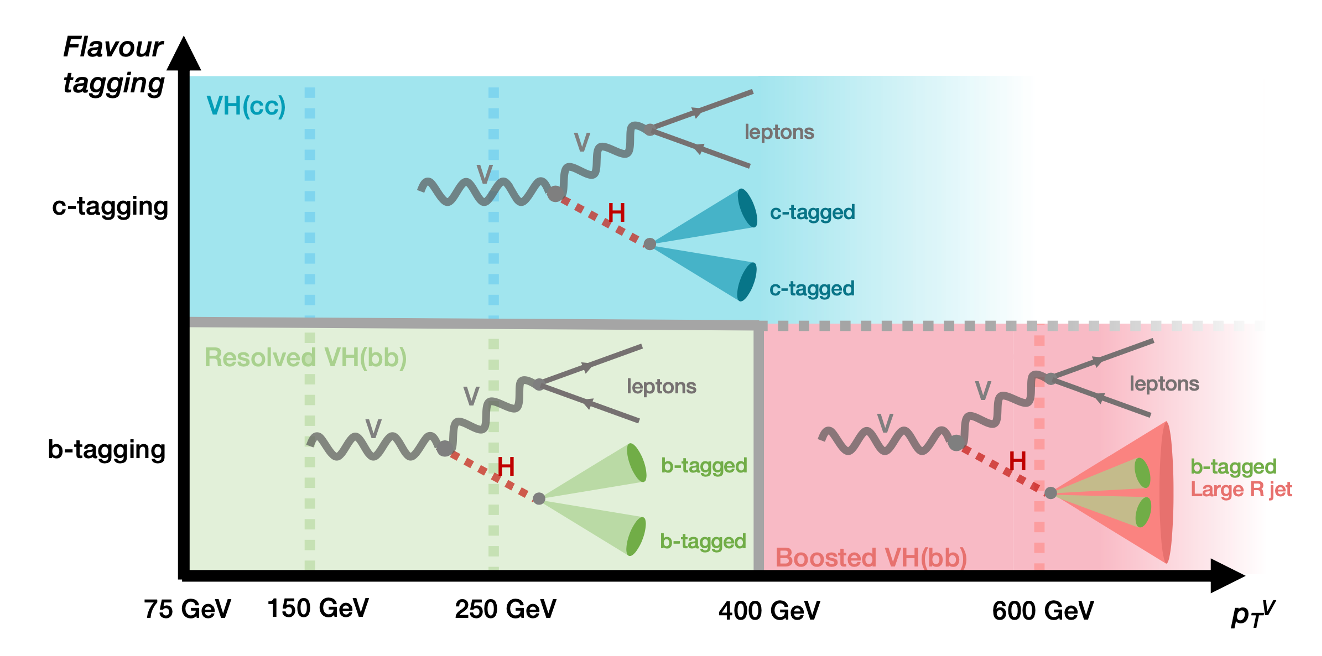
\includegraphics[width=\textwidth]{Images/VH/Cat/AnalysisRegime.png}
\caption{The analysis regimes considered in the combined $VH (H\rightarrow b\bar{b}/c\bar{c})$ analysis.} 
\label{fig:ana-strat}
\end{figure}

For each analysis regime, three channels are defined based on the decay mode of the vector boson $V$: $Z \rightarrow \nu \nu$ defines the \textit{0-lepton (0L)}, $W \rightarrow \ell \nu $ the \textit{1-lepton (1L)}, and $Z \rightarrow\ell^+\ell^-$ the \textit{2-lepton (2L)}, where $\ell$ refers to an electron or a muon and $\nu$ to a neutrino. The signals are the \vhb\ and \vhc\ processes, with the \gls{sm} diboson processes $VZ (Z\rightarrow b\bar{b})$ and $VZ (Z\rightarrow c\bar{c})$ considered as signals in a cross-check analysis. Having a larger cross section and being kinematically similar to the signals, these processes can be measured with good statistical significance and offer a test to verify the validity of the strategy adopted. The main backgrounds are the production of a vector boson with additional jets ($V$+jets) and the top-quark processes (\textit{Top}, predominantly the top-quark pair production $t\bar{t}$, with one of the $t$ decaying leptonically, and a sub-leading contribution from single top-quark production with an extra $W$ boson). Minor backgrounds are the \gls{qcd} multi-jet, the single-top process (without an associated $W$ boson) and non-signal diboson pair productions ($VV$). The processes are further described in the Section \ref{sec-datasets}. \\ 

Flavour tagging plays an essential role in the analysis, splitting the analysis phase space into different regimes. The most important backgrounds are also split based on flavour components. The $V+$jets is split into three components: $V+$ heavy flavour jets (\vhf, including $V+bb$ and $V+cc$), $V+$ mixed flavour (\vmf, including the $V+bc$, $V+bl$, and $V+cl$), and the $V+$ light flavours (\vlf, including all other possible flavour selection including $\tau$-leptons). The top-quark background is also split by flavour: the top$(bb)$, in which the two selected jets are $b$-tagged, is treated separately from the Top$(bq/qq)$ which groups all other flavours ($bc$, $bl$, and $qq$). The former is important in \vhb\ while the latter is the dominant flavour background in \vhc. The multi-jet is only included in the 1-lepton channel, as it is negligible in the other channels. \\

This chapter is separated into different sections introducing the datasets and \gls{mc} simulations (Section \ref{sec-datasets}), the object and event selection and categorisation (Section \ref{sec-selectionandcat}), the analysis discriminants (Section \ref{sec-vh-disc}) the experimental and processes modelling (Section \ref{sec-unc} and \ref{sec-mod}), the fit framework (Section \ref{subsec-likelidef}), and finally the main results (Section \ref{subsec-subsecVHBCfit}).

\section{Data and Simulated Samples}\label{sec-datasets} 
The combined analysis is performed on data collected during Run 2 of the \gls{lhc}, with proton-proton collisions recorded between 2015 and 2018 at a $\sqrt{s} = 13$ TeV for an integrated luminosity of 140.1 fb$^{-1}$ \cite{ATLAS:2022hro}. Data events passing quality requirements are selected, ensuring for example that all subdetectors were correctly operating. The analysis requires extensive and accurate \gls{mc} modelling of the signal and the background processes, except for the \gls{qcd} multi-jet and the \ttb\ background in the 2-lepton channel which have data-driven estimations. All \gls{mc} samples are simulated with the ATLAS detector \cite{ATLASSimulationInfra} using \textsc{Geant4} \cite{Agostinelli:602040}. The nominal samples are produced with the prescriptions described in Table \ref{tab:VHgenerators}, detailing the \gls{me} generators, \glsreset{ps}\gls{ps}, and \glsreset{pdf}\gls{pdf} releases used as well as the cross section precision. Samples are normalised either to the best theoretical cross section predictions or the generator cross sections. \\

\begin{table}
    \centering
    %\rotatebox{90}{
    \resizebox{\textwidth}{!}{
    \begin{tabular}{ l| l | l | l | l | l}
        \hline \hline
    Process & Matrix Element & PDF Set (ME) & Parton Shower & $\sigma$ order & $\sigma \times$ Br [pb] \\
     \hline \hline
     $qq \to WH \to \ell \nu b\bar{b}$ & PowHeg-Box v2 + GoSam + MiNLO & NNPDF3.0NLO & Pythia-8.245 & NNLO(QCD)+
    NLO(EW) & $2.69 \times 10^{-1}$ \\
     $qq \to ZH \to \nu \nu b\bar{b}$ & PowHeg-Box v2 + GoSam + MiNLO & NNPDF3.0NLO & Pythia-8.245 & NNLO(QCD)+
    NLO(EW) & $8.91 \times 10^{-2}$ \\
     $qq \to ZH \to \ell \ell b\bar{b}$ & PowHeg-Box v2 + GoSam + MiNLO & NNPDF3.0NLO & Pythia-8.245 & NNLO (QCD)+NLO(EW) & $4.48 \times 10^{-2}$ \\
     $gg \to ZH \to \nu \nu b\bar{b}$ & PowHeg-Box v2                   & NNPDF3.0NLO & Pythia-8.307 & NLO+NLL & $1.43 \times 10^{-2}$ \\
     $gg \to ZH \to \ell \ell b\bar{b}$ & PowHeg-Box v2                 & NNPDF3.0NLO & Pythia-8.307 & NLO+NLL & $7.23 \times 10^{-3}$ \\
     \hline
     $qq \to WH \to \ell \nu c\bar{c}$ & PowHeg-Box v2 + GoSam + MiNLO & NNPDF3.0NLO & Pythia-8.245 & NNLO(QCD)+
    NLO(EW) & $1.34 \times 10^{-2}$ \\
     $qq \to ZH \to \nu \nu c\bar{c}$ & PowHeg-Box v2 + GoSam + MiNLO & NNPDF3.0NLO & Pythia-8.245 & NNLO(QCD)+
    NLO(EW) & $4.42 \times 10^{-3}$ \\
     $qq \to ZH \to \ell \ell c\bar{c}$ & PowHeg-Box v2 + GoSam + MiNLO & NNPDF3.0NLO & Pythia-8.245 & NNLO (QCD)+NLO(EW) & $2.23 \times 10^{-3}$ \\
     $gg \to ZH \to \nu \nu c\bar{c}$ & PowHeg-Box v2                   & NNPDF3.0NLO & Pythia-8.307 & NLO+NLL & $7.10 \times 10^{-4}$ \\
     $gg \to ZH \to \ell \ell c\bar{c}$ & PowHeg-Box v2                 & NNPDF3.0NLO & Pythia-8.307 & NLO+NLL & $3.59 \times 10^{-4}$ \\
    % \hline
    %  $Z \to \nu \nu$ + jets   & Sherpa 2.2.1 & NNPDF3.0NNLO & Sherpa 2.2.1 & NNLO & 10700 \\
    %  $W \to \ell \nu$ + jets  & Sherpa 2.2.1 & NNPDF3.0NNLO & Sherpa 2.2.1 & NNLO & 60200 \\
    %  $Z \to \ell \ell$ + jets & Sherpa 2.2.1 & NNPDF3.0NNLO & Sherpa 2.2.1 & NNLO & 6300 \\
      \hline
      $W \to \ell \nu$ + jets  & Sherpa 2.2.11 & NNPDF3.0NNLO & Sherpa 2.2.11 & NNLO & 60242  \\
      $Z \to \ell \ell$ + jets & Sherpa 2.2.11 & NNPDF3.0NNLO & Sherpa 2.2.11 & NNLO & 6201   \\
      $Z \to \nu \nu$ + jets   & Sherpa 2.2.11 & NNPDF3.0NNLO & Sherpa 2.2.11 & NNLO & 416.05  \\
      \hline
      \ttb   & Powheg-Box v2 & NNPDF3.0NLO & Pythia-8.230 & NNLO+NNLL &  704  \\
      single-top ($Wt$)  & Powheg-Box v2 & NNPDF3.0NLO & Pythia-8.230 & Approx. NNLO & 80.03  \\
      single-top ($t$)   & Powheg-Box v2 & NNPDF3.0NLO & Pythia-8.230 & NLO       & 70.7  \\
      single-top ($s$)   & Powheg-Box v2 & NNPDF3.0NLO & Pythia-8.230 & NLO       & 3.35  \\
    %  \hline
    %  $qq \to WW$ & Sherpa 2.2.1 & NNPDF3.0NNLO & Sherpa 2.2.1 & NLO & 45.7 \\
    %  $qq \to WZ$ & Sherpa 2.2.1 & NNPDF3.0NNLO & Sherpa 2.2.1 & NLO & 21.7 \\
    %  $qq \to ZZ$ & Sherpa 2.2.1 & NNPDF3.0NNLO & Sherpa 2.2.1 & NLO & 6.53 \\
      \hline
      $qq \to WW$ & Sherpa 2.2.11 & NNPDF3.0NNLO & Sherpa 2.2.11 & NLO & 47.93 \\
      $qq \to WZ$ & Sherpa 2.2.11 & NNPDF3.0NNLO & Sherpa 2.2.11 & NLO & 20.85 \\
      $qq \to ZZ$ & Sherpa 2.2.11 & NNPDF3.0NNLO & Sherpa 2.2.11 & NLO & 6.33 \\
      $gg \to VV$ & Sherpa 2.2.2 & NNPDF3.0NNLO  & Sherpa 2.2.2 & NLO & 2.78 \\
     \hline \hline
    \end{tabular}
    }
    \caption{The nominal Monte Carlo samples used in the \vhbc\ analysis, and the corresponding process cross-sections at $\sqrt{s} = 13$ TeV. The PDF sets in the table are the ones used for the matrix element.}
    \label{tab:VHgenerators}
\end{table}
    

Both simulated samples and data are reconstructed with the ATLAS offline reconstruction software \cite{ATL-SOFT-PUB-2021-001}. The \textsc{EvtGen} 1.6.0 program is used to simulate the properties of $b$- and $c$-hadrons decays\footnote{\textsc{EvtGen} 1.7.0 is used for the \textsc{Sherpa} generated samples.} \cite{LANGE2001152}. Pile-up is included in the simulation, both from multiple interactions in the same and adjacent bunch crossing. This is performed by overlaying events with minimum bias simulated using \textsc{\textsc{Pythia}} 8 with A3 tune and interfaced with the \textsc{NNPDF} 2.3 \glspl{pdf} \cite{SJOSTRAND2015159}. The rest of this section gives more details about the simulation of the different processes. When relevant, alternative samples generated from a different setup to the nominal samples are introduced. These alternative samples are used to assess modelling uncertainties in Section \ref{sec-modStrat}, as summarised in Table~\ref{tab:summary_altsamples}.

\subsection{Signal Processes}
The analysis targets the \vhb\ and \vhc\ processes as \textit{signals}. The Leading Order (LO) Feynman diagrams contributing to the associated production $VH$ are the $qq$-initiated modes depicted in Figure~\ref{fig:feynloVH}. A gluon-initiated production of $ZH$ is also possible at Next-to-Leading Order (NLO) with a quark loop (mostly top-quark), as depicted in Figure~\ref{fig:feynnloVH}. The \glsreset{me}\gls{me} calculations are based on the \textsc{Powheg-Box v2} generator \cite{StefanoFrixione_20072, POWHEGBOX}. The $qq$-initiated $VH$ samples are simulated with the \textsc{Powheg} generator with the multiscale improved NLO (\textsc{MiNLO}) procedure \cite{powhegHW}, with one-loop amplitudes computed with the GoSam automated software \cite{gosam}. The $qq$-initiated samples simulate \glsreset{ps}\gls{ps}, \glsreset{ue}\gls{ue}, and multiple parton interactions with \textsc{Pythia} 8.245, while the $gg$-initiated use \textsc{Pythia} 8.307 \cite{SJOSTRAND2015159}. Both use the AZNLO tune \cite{measureZGboson} with \glspl{pdf} based on the \textsc{NNPDF3.0NLO} for matrix elements \cite{PDFLHCrun2}. \\

\begin{figure}[h!]
  \center
  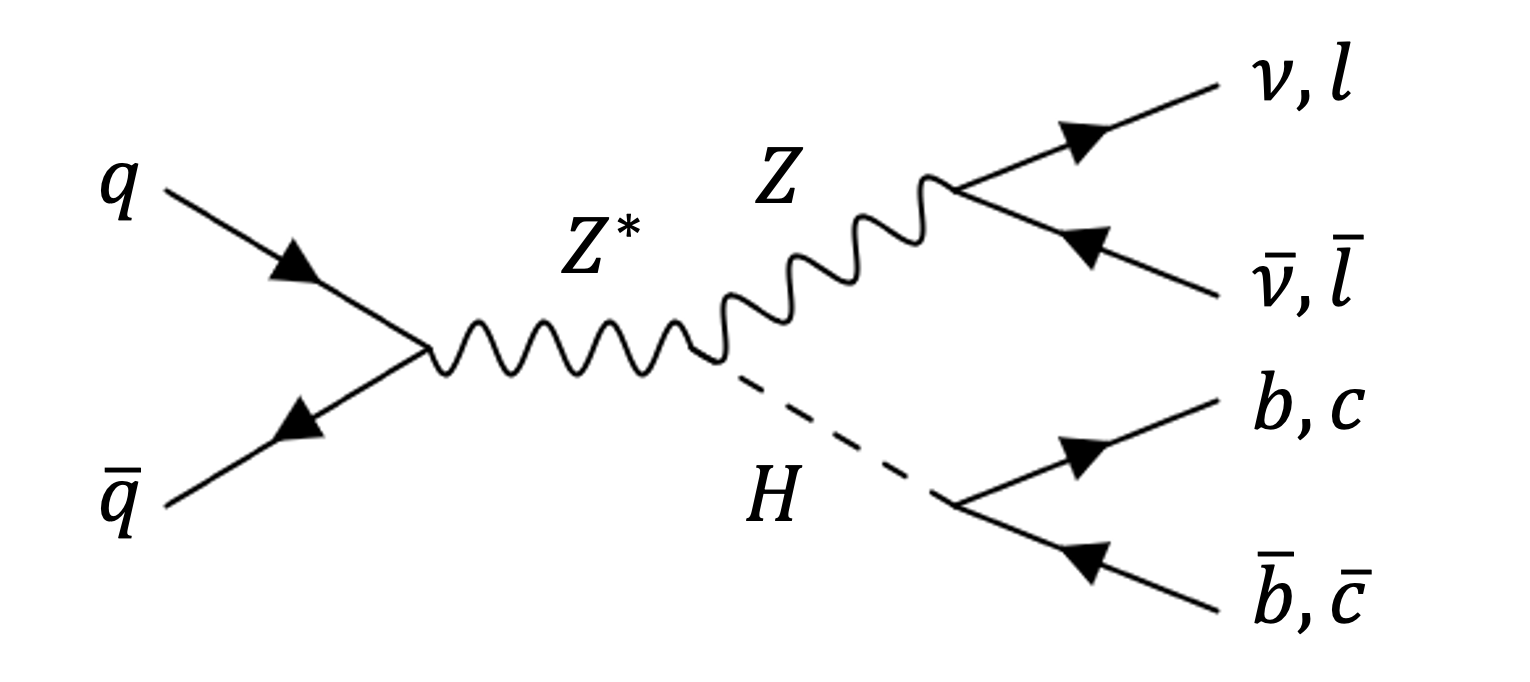
\includegraphics[width=0.48\textwidth]{Images/VH/Feynman/zh.png}
  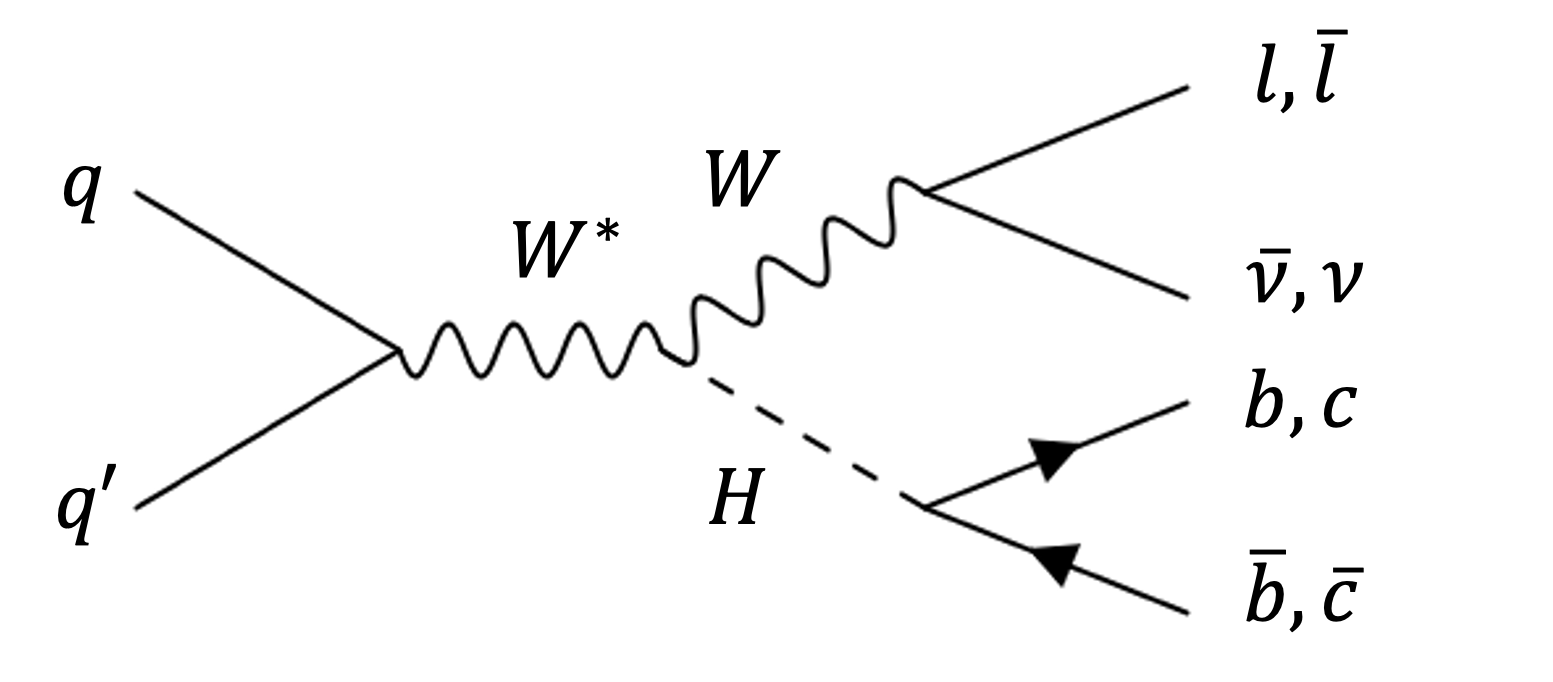
\includegraphics[width=0.48\textwidth]{Images/VH/Feynman/wh.png}
  \caption{Leading order Feynman diagrams for the $qq$-initiated \vhbc.} 
  \label{fig:feynloVH}
\end{figure}

\begin{figure}[h!]
  \center
  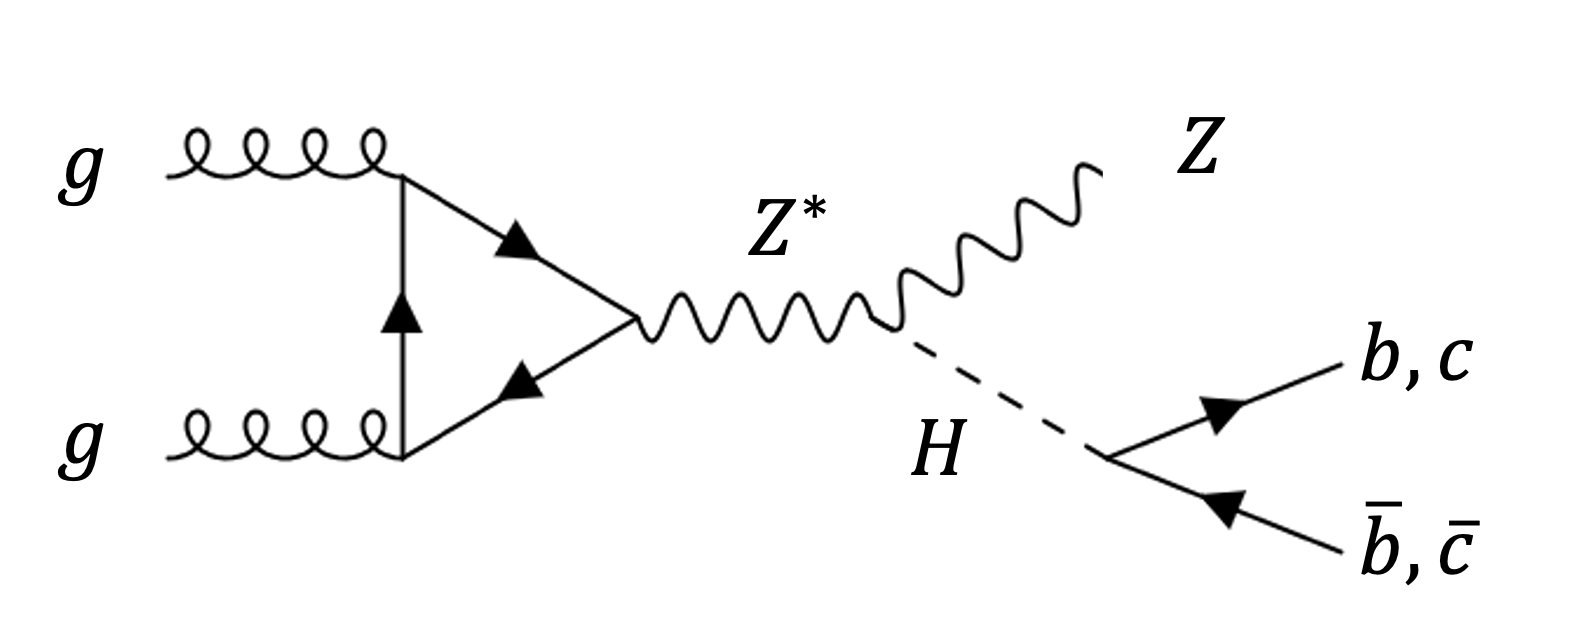
\includegraphics[width=0.48\textwidth]{Images/VH/Feynman/vh2order.png}
  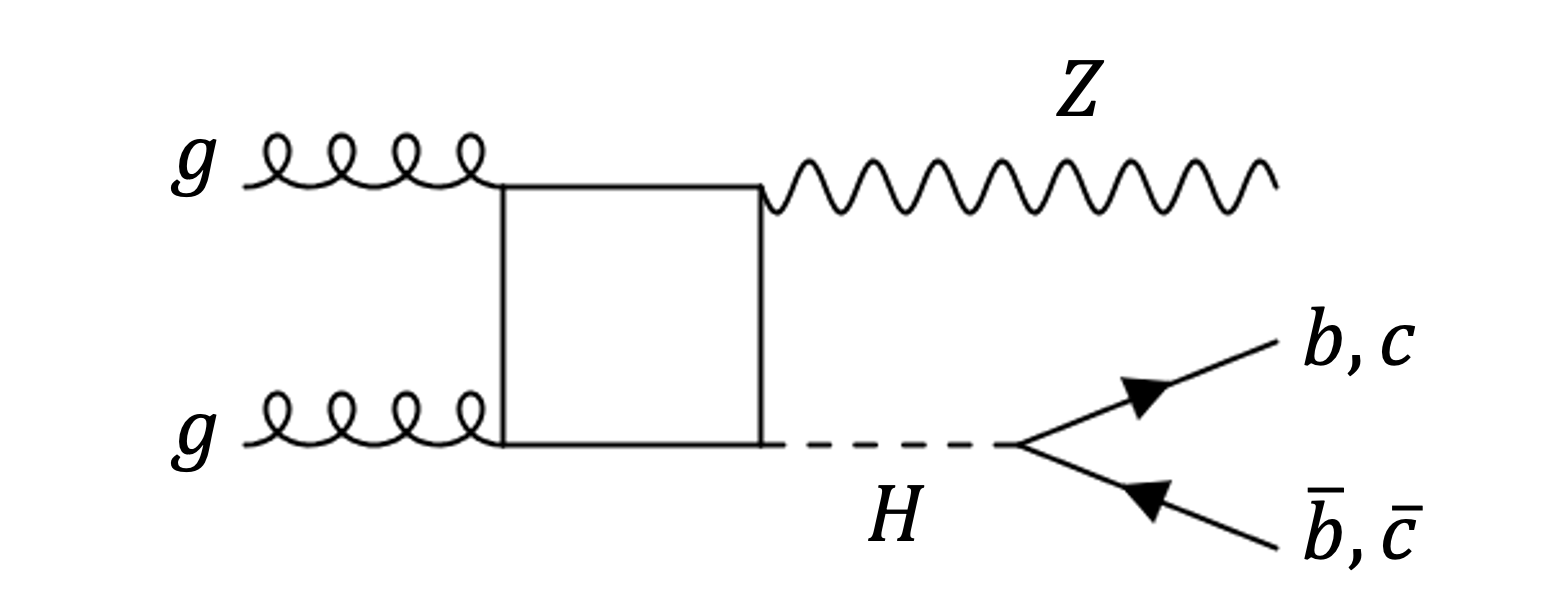
\includegraphics[width=0.48\textwidth]{Images/VH/Feynman/vh3order.png}
  \caption{Feynman diagrams of the $gg$-initiated contributions to $ZH(H\rightarrow b\bar{b}/c\bar{c})$.} 
  \label{fig:feynnloVH}
\end{figure}

The inclusive cross sections for $WH$ and $ZH$ are calculated at NNLO in \gls{qcd} \cite{BREIN2004149} and NLO in \glsreset{ew}\gls{ew} \cite{PDFLHCrun2}. The $gg$-initiaed $ZH$ contribution relies on the LO prediction from \textsc{Powheg} instantiated with \textsc{Pythia} 8.

\paragraph{Alternative samples} are simulated with \textsc{Powheg}+\textsc{MiNLO}+\textsc{Herwig} 7.0 \cite{bellm2017herwig}, with the same simulation stack as the nominal samples but replacing \textsc{Pythia} 8 by \textsc{Herwig} 7.0 for the simulation of the \gls{ps}, hadronisation, \gls{ue}, and multiple parton interactions.

\subsection{Background Processes}
\subsubsection{$\boldsymbol{V+}$jets}
The production of a gauge vector boson $V$ in association with jets is the largest background in the analysis. Some leading contributing Feynman diagrams to this process are presented in Figure~\ref{fig:feynVJ}. Both the $Z+$jets and $W+$jets are simulated with \textsc{Sherpa} 2.2.11 \cite{10.21468/SciPostPhys.7.3.034}, which delivers NLO precision on \gls{me} computation for up to 2 jets and LO accuracy for between 3 and 5 jets. \gls{ps} and hadronisation are treated by the default \textsc{Sherpa} generator, with the NNLO \glspl{pdf} based on NNPDF3.0NNLO \cite{PDFLHCrun2}. Uncertainties from missing higher orders are evaluated by varying the \gls{qcd} renormalisation and factorisation scales $\mu_R$ and $\mu_F$ in the matrix elements by respective factors 0.5 and 2. Flavour filtering is applied to generate samples enriched with heavy-flavour quarks.

\begin{figure}[h!]
  \center
  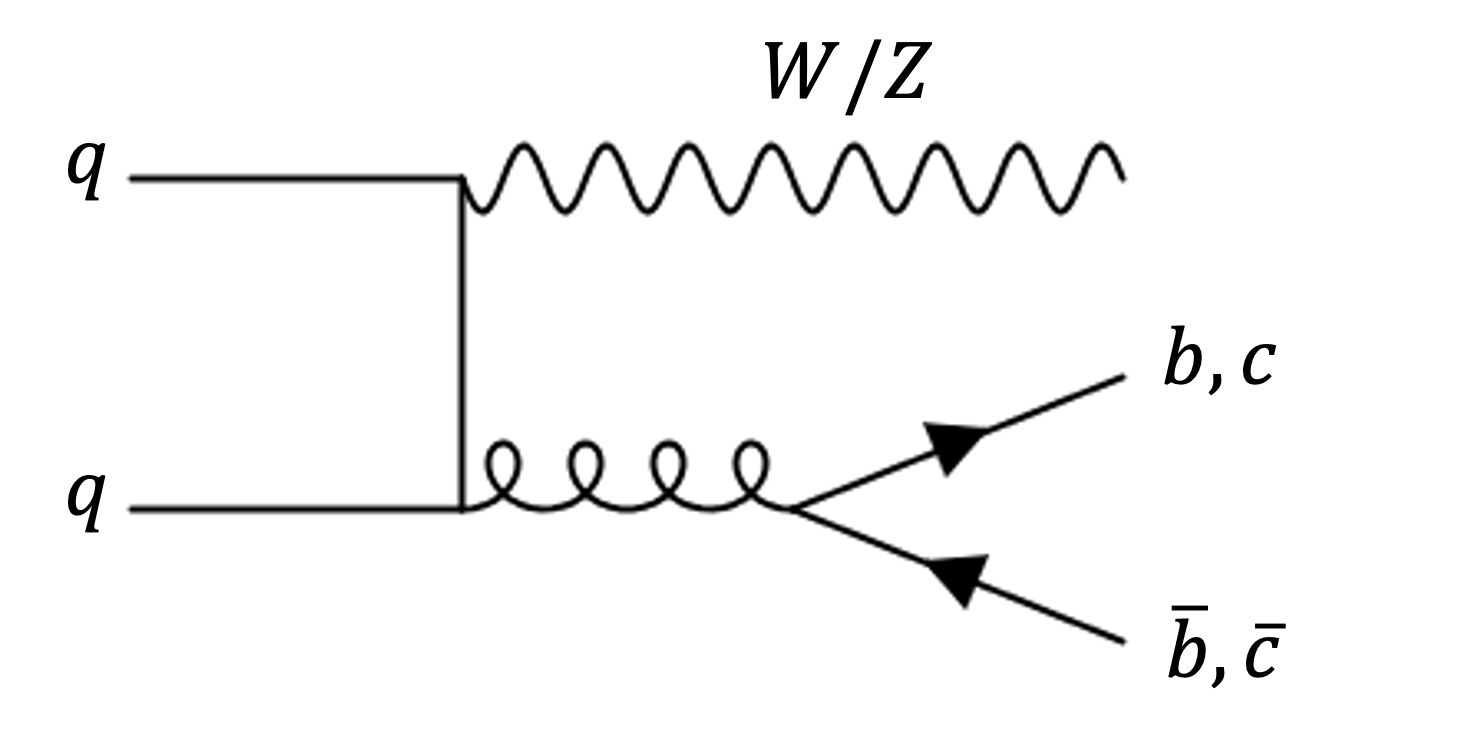
\includegraphics[width=0.48\textwidth]{Images/VH/Feynman/vjet.png}
  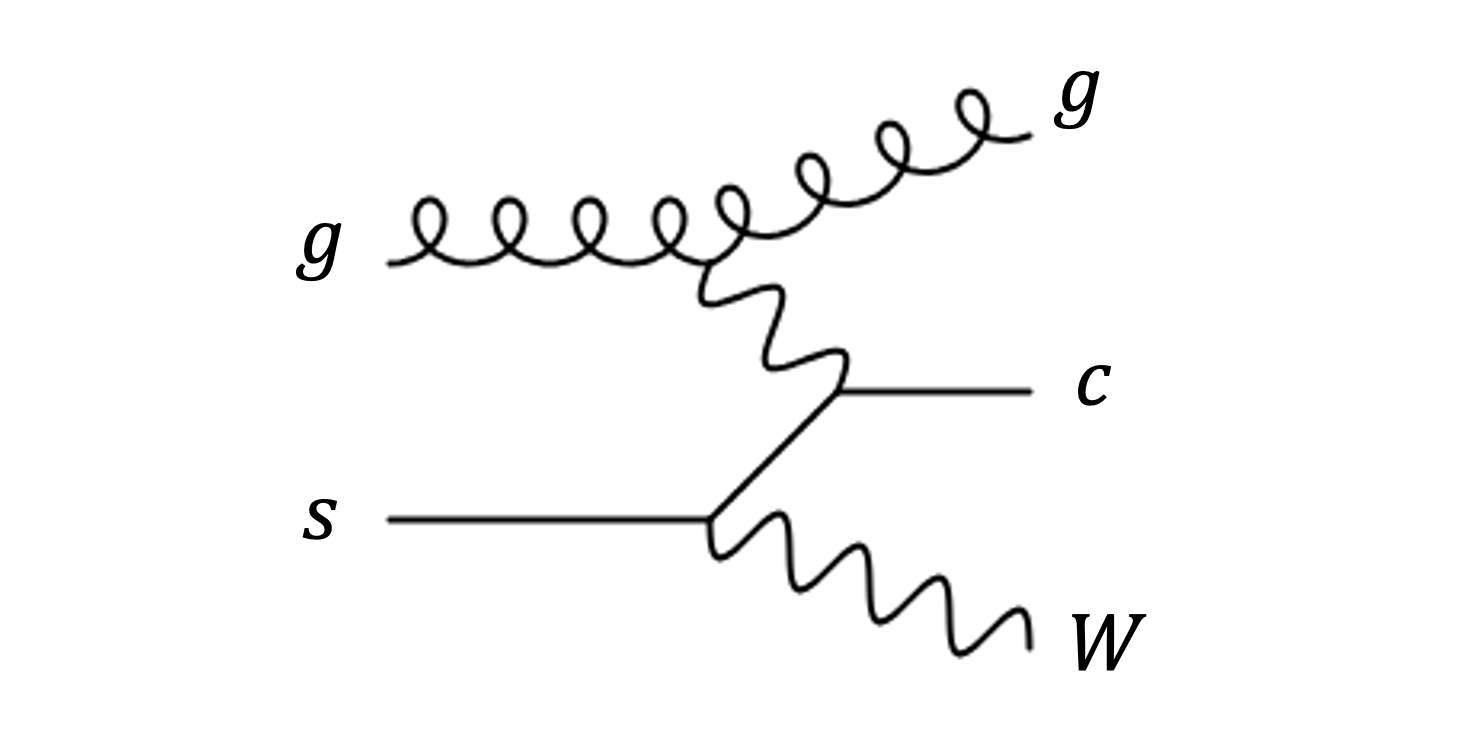
\includegraphics[width=0.48\textwidth]{Images/VH/Feynman/vjet2.png}
  \caption{Leading order Feynman diagrams of the $V+$jets process. The left diagram gives jet pairs of the same flavour due to the gluon splitting, while the right one can give mixed flavours.} 
  \label{fig:feynVJ}
\end{figure}

\paragraph{Alternative samples} Two sets of alternative samples are available:
\begin{itemize}
  \item \textsc{MadGraph FxFx} \cite{Frederix:2012ps} samples are produced for the modelling studies, using the \textsc{MadGraph5\_aMC@NLO} 2.6.5 program \cite{madgraph}. This generates events with $V$ boson and up to three additional partons in the final state at NLO accuracy. The scales $\mu_R$ and $\mu_F$ are set to 1/2 the transverse mass of all final-state partons + leptons. \textsc{Pythia} 8.240 is interfaced for \gls{ps} and hadronisation, with the A14 tune \cite{ATL-PHYS-PUB-2014-021} and the NNPDF2.3LO \gls{pdf} \cite{BALL2013244} set with $\alpha_s = 0.13$.
  \item \textsc{Sherpa} 2.2.1 \cite{sherpa2.2paper} samples are used as alternative as they give different \ptv\ distributions to \textsc{Sherpa} 2.2.11 \cite{simVjet}, an important modification given the observed data-\gls{mc} disagreements in the \ptv\ distributions.
\end{itemize}

\subsubsection{Top-pair Production}\label{subsec-vh-top-samples}
The \ttb\ process is the second most important background in the analysis. The leading order Feynman diagram for this process is shown in Figure \ref{fig:feynttb}. The nominal samples are generated for the 0L and 1L channels with \textsc{Powheg} at NLO calculation of the matrix element \cite{StefanoFrixione_2007, PaoloNason_2004}. It is interfaced with \textsc{Pythia} 8.230 with the NNPDF3.0NLO \glspl{pdf} using the A14 tune for \gls{ps}, hadronisation, and \gls{ue} description. Filtering is applied while simulating to enhance statistics. Cross sections are calculated to NNLO in \gls{qcd}, with resummation of the Next-to-Next-to-Leading Logarithmic (NNLL) soft-gluon terms \cite{CZAKON20142930}.

\begin{figure}[h!]
  \center
  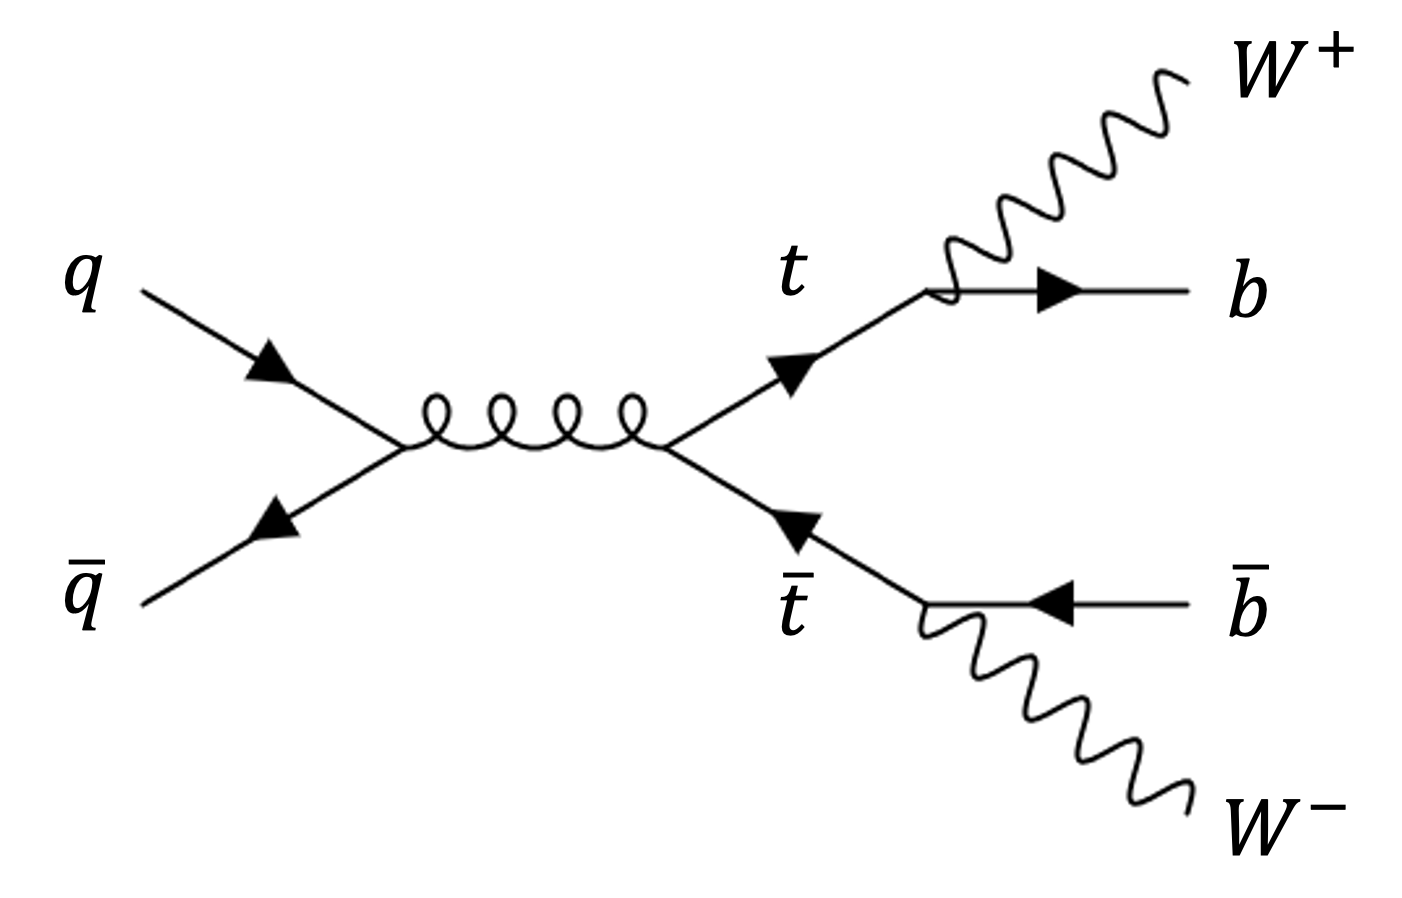
\includegraphics[width=0.5\textwidth]{Images/VH/Feynman/ttb.png}
  \caption{Feynman diagrams of the \ttb\ production and decay.} 
  \label{fig:feynttb}
\end{figure}

\paragraph{Alternative samples} Several alternatives are simulated for modelling studies:
\begin{itemize}
  \item Replacing \textsc{Pythia} by \textsc{Herwing} 7.0 with H7UE tune \cite{herwig7R} while keeping the same nominal \textsc{Powheg} setup. This sample is used to systematically assess variations to the parton shower, hadronisation, and underlying event modelling.
  \item Replacing \textsc{Powheg} by \textsc{MadGraph5\_aMC@NLO} \cite{madgraph} for NLO hard scattering matrix element modelling with the nominal \textsc{Pythia} for \gls{ps}, hadronisation, and the \gls{ue} simulation. This sample is used to systematically assess variation in the matrix element prediction.
  \item Weights variations tuning the \glsreset{isr}\gls{isr} and \glsreset{fsr}\gls{fsr} contributions relative to the nominal setup. There are 4 such variations, based on the nominal \textsc{Powheg} + \textsc{Pythia} 8.230:
  \begin{itemize}
    \item High- / low-variations of \gls{isr}, where the $\mu_R$ and $\mu_F$ scales are halved / doubled. %\footnote{For the high variation, the \textit{hdamp} parameter is doubled from its nominal value of 1.5 $\times$ $m_{\text{top}}$.}.
    \item Up- / down-variations of \gls{fsr}, obtained by halving / doubling the renormalisation scale $\mu_{R}$. 
  \end{itemize}
\end{itemize} 

\subsubsection{Single-top Production}
The single-top process combines different channels, with the leading Feynman diagrams depicted in Figure~\ref{fig:feynstop}. The dominant contribution is the associated top-production $Wt$ channel, with the $t \rightarrow Wb$. The two other contributions are the $t$- and $s$-channel, with the former having a larger cross section than the $s$-channel. These processes are simulated similarly to the \ttb, with the cross sections calculated for a top-quark mass of $m_t = 172.5$ GeV at NLO in \gls{qcd} for the $t$- and $s$-channels \cite{ALIEV20111034, KANT201574}, and with approximate NNLO accuracy from NNLL soft-gluon resummation for the fiducial $Wt$ production cross section \cite{PhysRevD.82.054018, kidonakis2013quark}.
\begin{figure}[h!]
  \center
  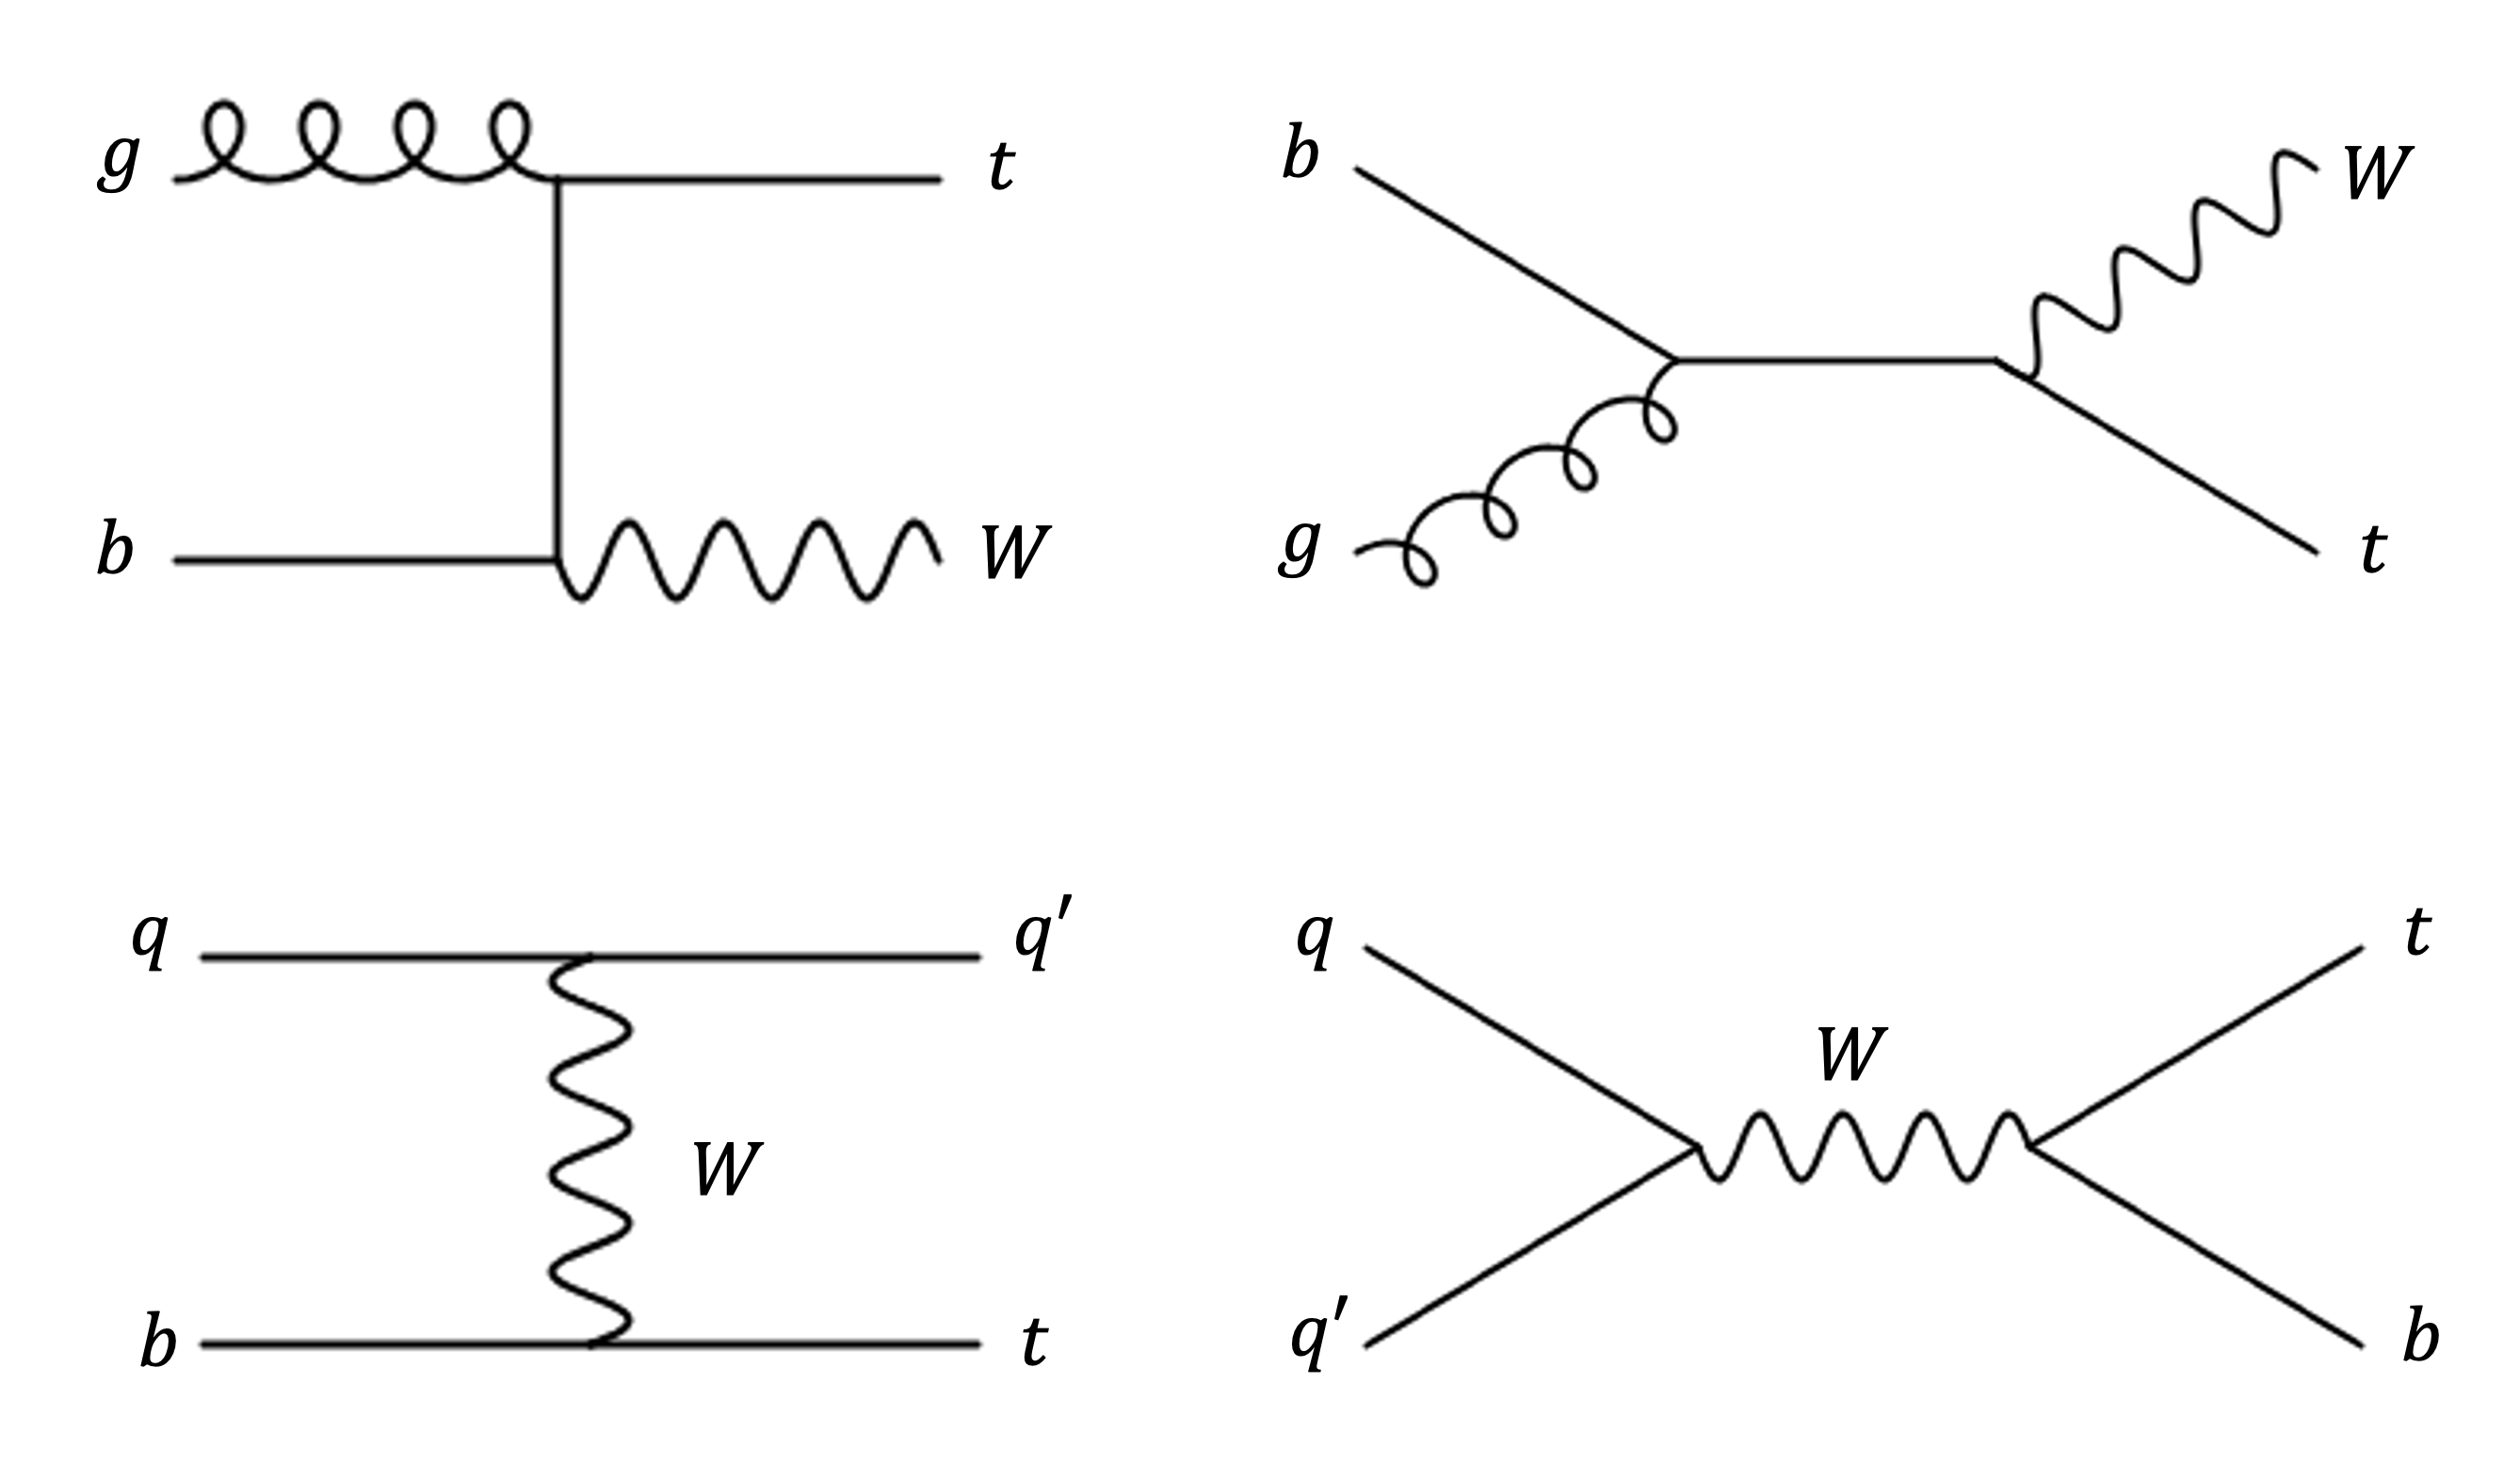
\includegraphics[width=0.7\textwidth]{Images/VH/Feynman/singletop.png}
  \caption{Feynman diagrams of the $Wt$-production (top) and the single top production (bottom) in the $t$-channel (left) and the $s$-channel (right).} 
  \label{fig:feynstop}
\end{figure}

The $Wt$ production has diagrams overlapping with the \ttb\ production at NLO in \gls{qcd}. In the analysis, a diagram subtraction (\textit{DS}) scheme is applied to remove the overlap with \ttb\ by locally cancelling the \ttb\ contributions in the NLO $Wt$ cross section calculation \cite{StefanoFrixione_2008}. 

\paragraph{Alternative samples} are produced for the single-top $Wt$- and $t$-channels\footnote{No alternatives are derived for the single-top $s$-channel due to its small contribution in the analysis.}:
\begin{itemize}
  \item The 2 alternative generators and the 4 changes to the \gls{isr} and \gls{fsr} used for the alternatives of \ttb\ are also applied to the $Wt$- and $t$-channels.
  \item For $Wt$ only, a sample using a different overlap removal procedure is produced with the diagram removal (\textit{DR}) scheme \cite{StefanoFrixione_2008} to systematically model the overlap with \ttb. This scheme removes the diagrams in the NLO $Wt$ amplitudes that are doubly-resonant, when both $t$-quark are on-shell. $DR$ was the default scheme in prior iterations of this analysis, but the $DS$ samples showed better agreement with data in the boosted regime.
\end{itemize}

\subsubsection{Diboson Process}
The diboson processes $WW$, $WZ$, and $ZZ$ enter the analysis both as a background, with a hadronically decaying $V$ boson mistaken for the Higgs, and as a cross-check signal when decaying into a $b\bar{b}$ or $c\bar{c}$ pair. Some leading $qq$-initated Feynman diagrams are depicted in Figure \ref{fig:feyndiV}, with gluon-initiated diagrams also possible via quark-loops. The $qq$-initiated diboson samples are simulated similarly to the $V+$jets, using \textsc{Sherpa} 2.2.11 \cite{10.21468/SciPostPhys.7.3.034}. The $gg$-initiated processes are simulated with the older \textsc{Sherpa} 2.2.2 version. The cross sections are computed at NLO precision, with the NNLO \glspl{pdf} based on NNPDF3.0NNLO \cite{PDFLHCrun2} for both the matrix element and parton shower.
\begin{figure}[h!]
  \center
  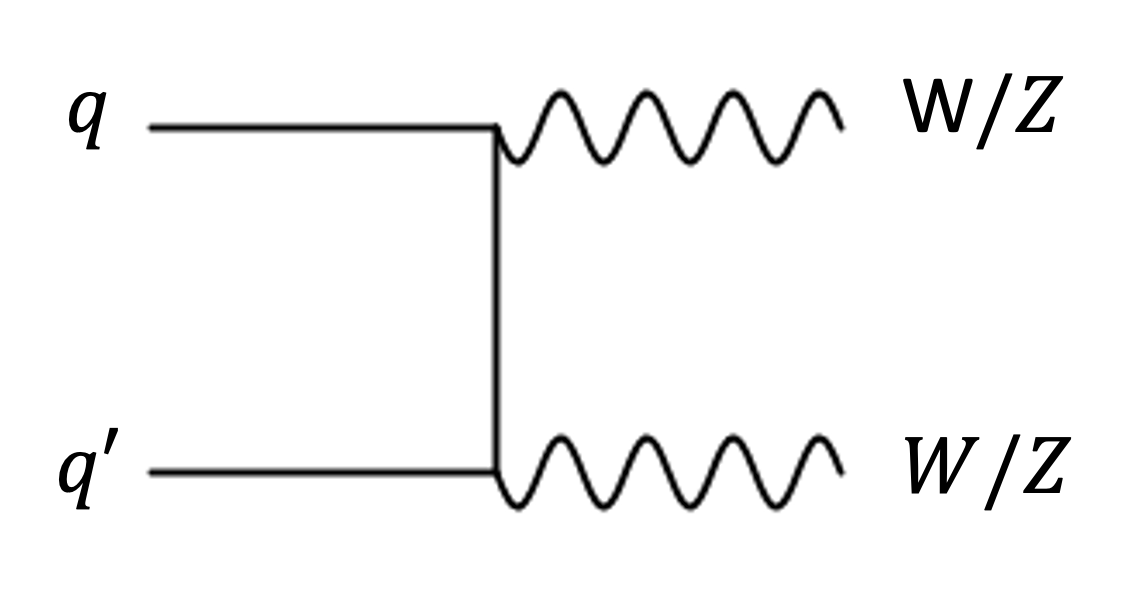
\includegraphics[width=0.32\textwidth]{Images/VH/Feynman/diboson.png}
  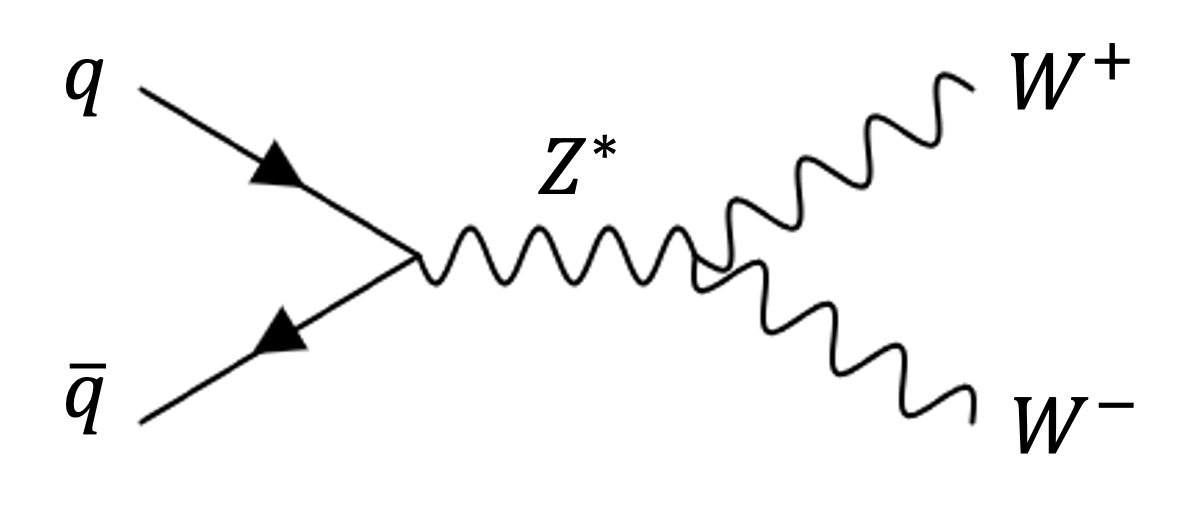
\includegraphics[width=0.32\textwidth]{Images/VH/Feynman/diW.png}
  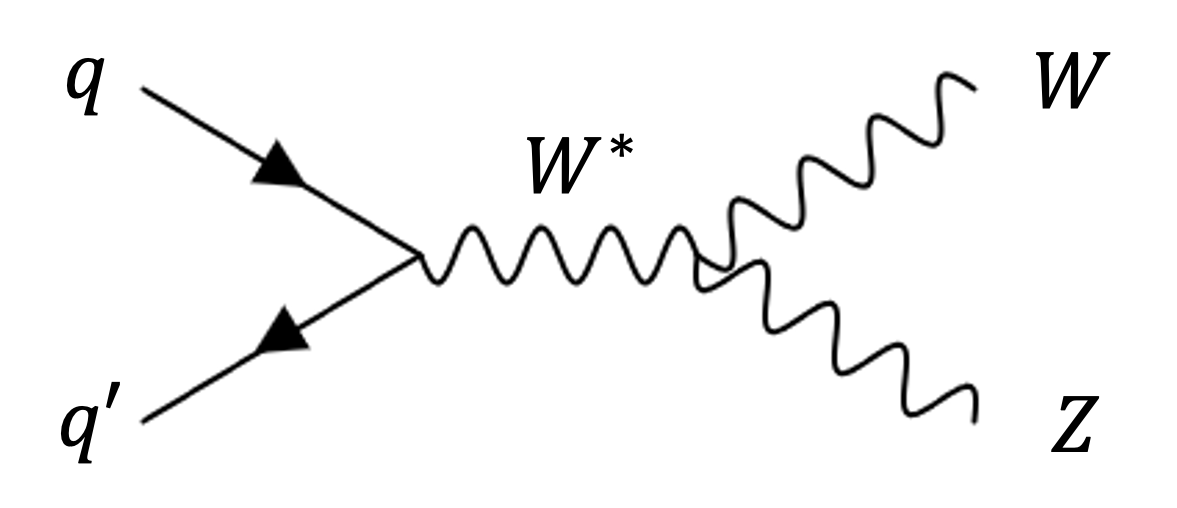
\includegraphics[width=0.32\textwidth]{Images/VH/Feynman/diWZ.png}
  \caption{Feynman diagrams of the diboson production in the $t$- (left) and $s$-channel (centre \& right). The $t$-channel can lead to any combination of $W$ and $Z$ depending on the initial quark-pair.}
  \label{fig:feyndiV}
\end{figure}

\paragraph{Alternative samples:}
\begin{itemize}
  \item \textsc{Powheg} v2 interfaced with \textsc{Pythia} 8 samples are produced to systematically assess \gls{me} and \gls{ps} variations. 
  \item \textsc{Sherpa} 2.2.1 samples are produced to systematically model the impact of varying the fragmentation function. 
\end{itemize}

\subsubsection{QCD Multi-jet}
This process is estimated from data instead of simulations because of the difficulty in generating sufficient statistics samples due to the low selection efficiency, despite having a much larger production cross section than the Higgs. \gls{qcd} multi-jet events can be selected when heavy-flavour hadrons decay semi-leptonically or jets are misidentified as leptons. Such leptons are normally not isolated, and only a small fraction passes the lepton requirements. The multi-jet is negligible in the 0-lepton and 2-lepton channels thanks to the strict selections available. In the 1-lepton resolved channel, the remaining contribution is assessed from data-driven templates for \vhb\ or as a side control region for \vhc. In both cases, a region enriched in multi-jet is defined by inverting the lepton isolation requirements. The residual multi-jet is mostly present at low \ptv\ values and is therefore ignored in the boosted regime.

%In the template method, the shape of the multi-jet is derived in a special control region \textit{mjCR} enriched in \gls{qcd} events, with the multi-jet normalisation factor free-floated in the signal region fit. Independent template fits are performed for the electron and muon channels in the low and medium \ptv\ regions\footnot{Respectively $[75, 150]$ GeV, and $[150, 400]$ GeV.}, for 2- and 3-jet categories separately. The mjCR is obtained by inverting some of the tight isolation cuts for the lepton and requiring only 1 $B$-tag to increase statistics. The distribution of $m_T^W$ in the mjCR is used in the fit as it gives the best discrimination between multi-jet and the other processes. Indeed, the main other backgrounds in the mjCRs are the $W+$jets and \ttb, which both have a characteristic peak close to the $W$ mass while the multi-jet has a smoothly falling distribution.
